\documentclass[../../DD.tex]{subfiles}
\begin{document}
	\section{Use case scenarios}
		Use case scenarios help to focus on the needs of the users. They provide a way of understanding the user's behaviour and interaction with the application. This helps the designers create intuitive navigation structures according to the needs of the users, organize the web content and define the functional requirements of the website.
  
		\subsection{Use case 1}
        Samantha is a young software engineer with a strong background in financial field. She has been working for two years as software engineer in Bending Spoons.

        For this reason, she wants to understand first what does the company, and in which field they work in and moreover where she will have the possibility to work. Everything can be found in the homepage (see \ref{fig: UC01}).

        \begin{figure}[!htb]
            \centering
            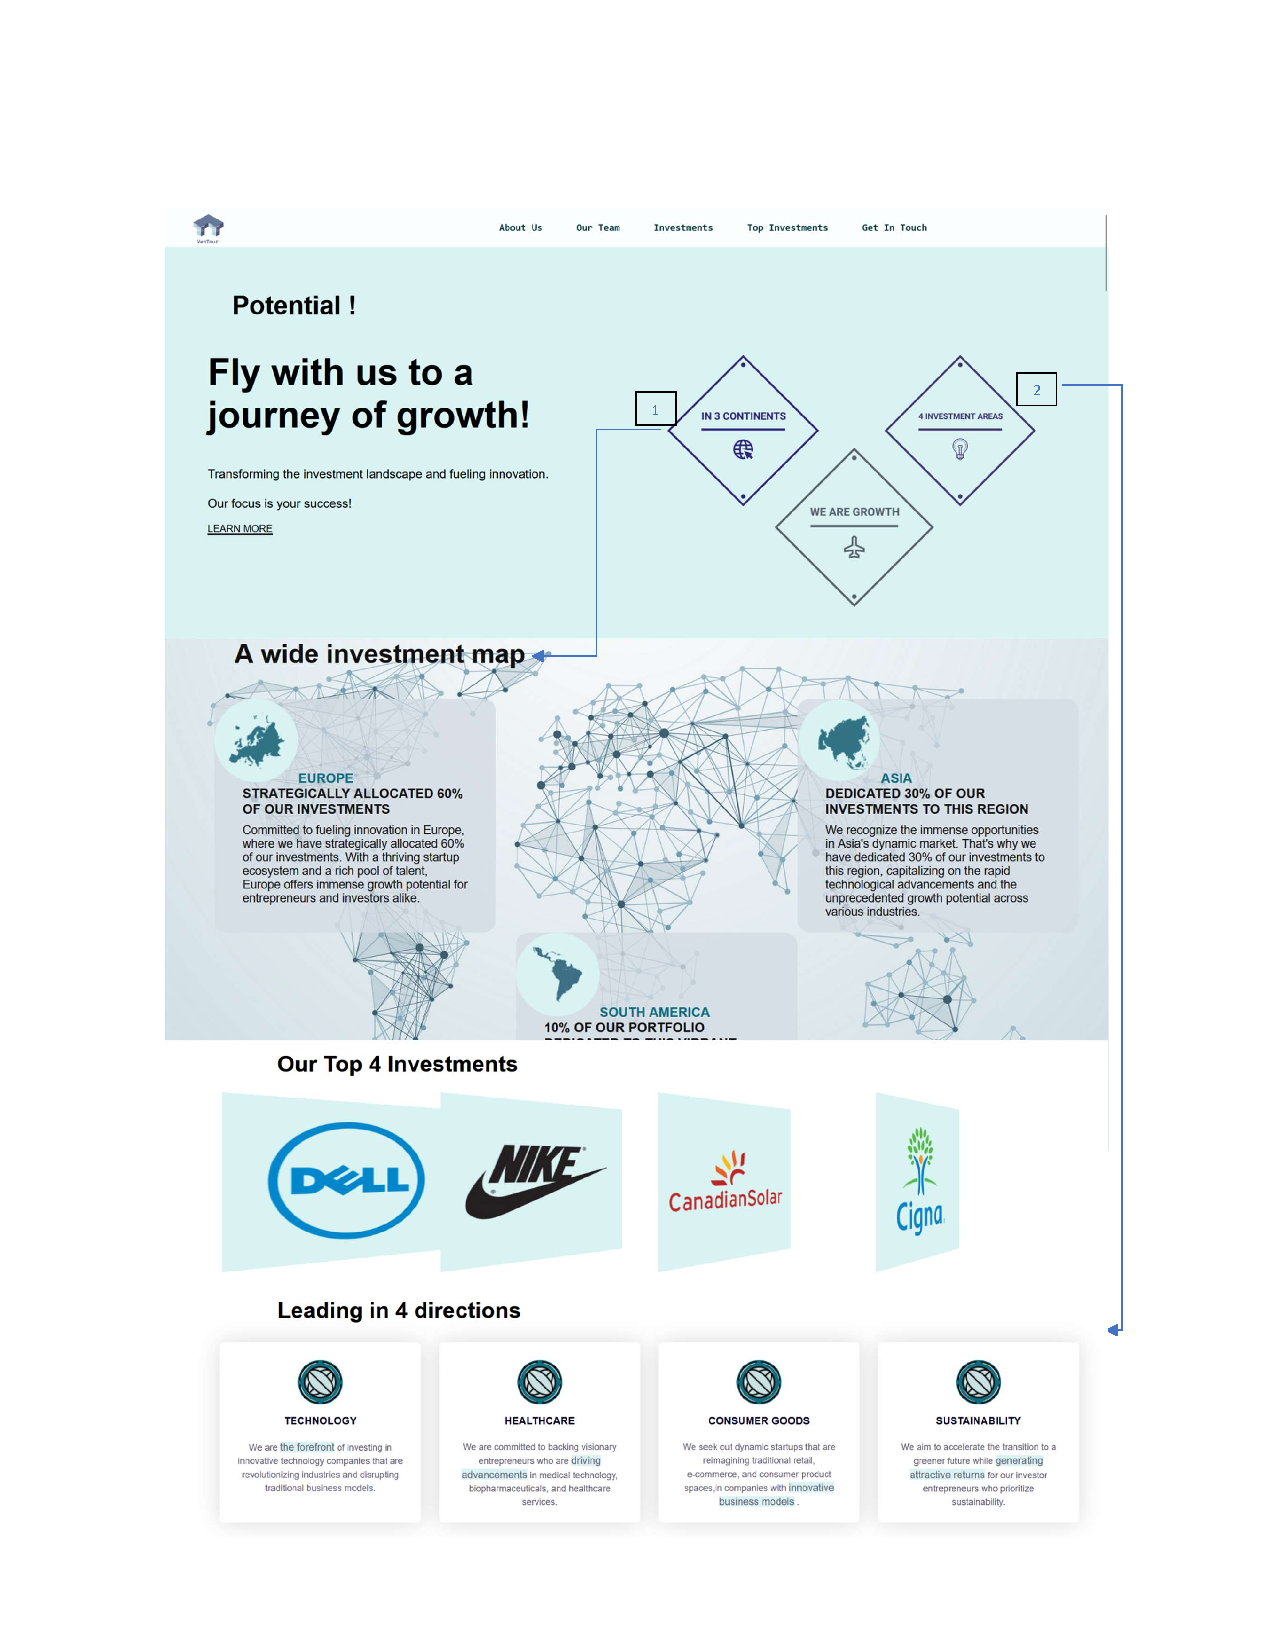
\includegraphics[width=\textwidth]{Images/scenarios/Use Case 1.pdf}
            \caption{Samantha first of all is in the Home page and browse the home page}
            \label{fig: UC01}
        \end{figure}
    
        Once she has understood the potentiality of Ventour, she wants to see if there are some open position to work in the company. To do it, she goes in \textit{"Get in touch"} and she looks for open position. 
        She finds one open position as Frontend developer and she decides to apply, sending an email thanks to the form provided by the website (see \ref{fig: UC02}).

        \begin{figure}[!htb]
            \centering
            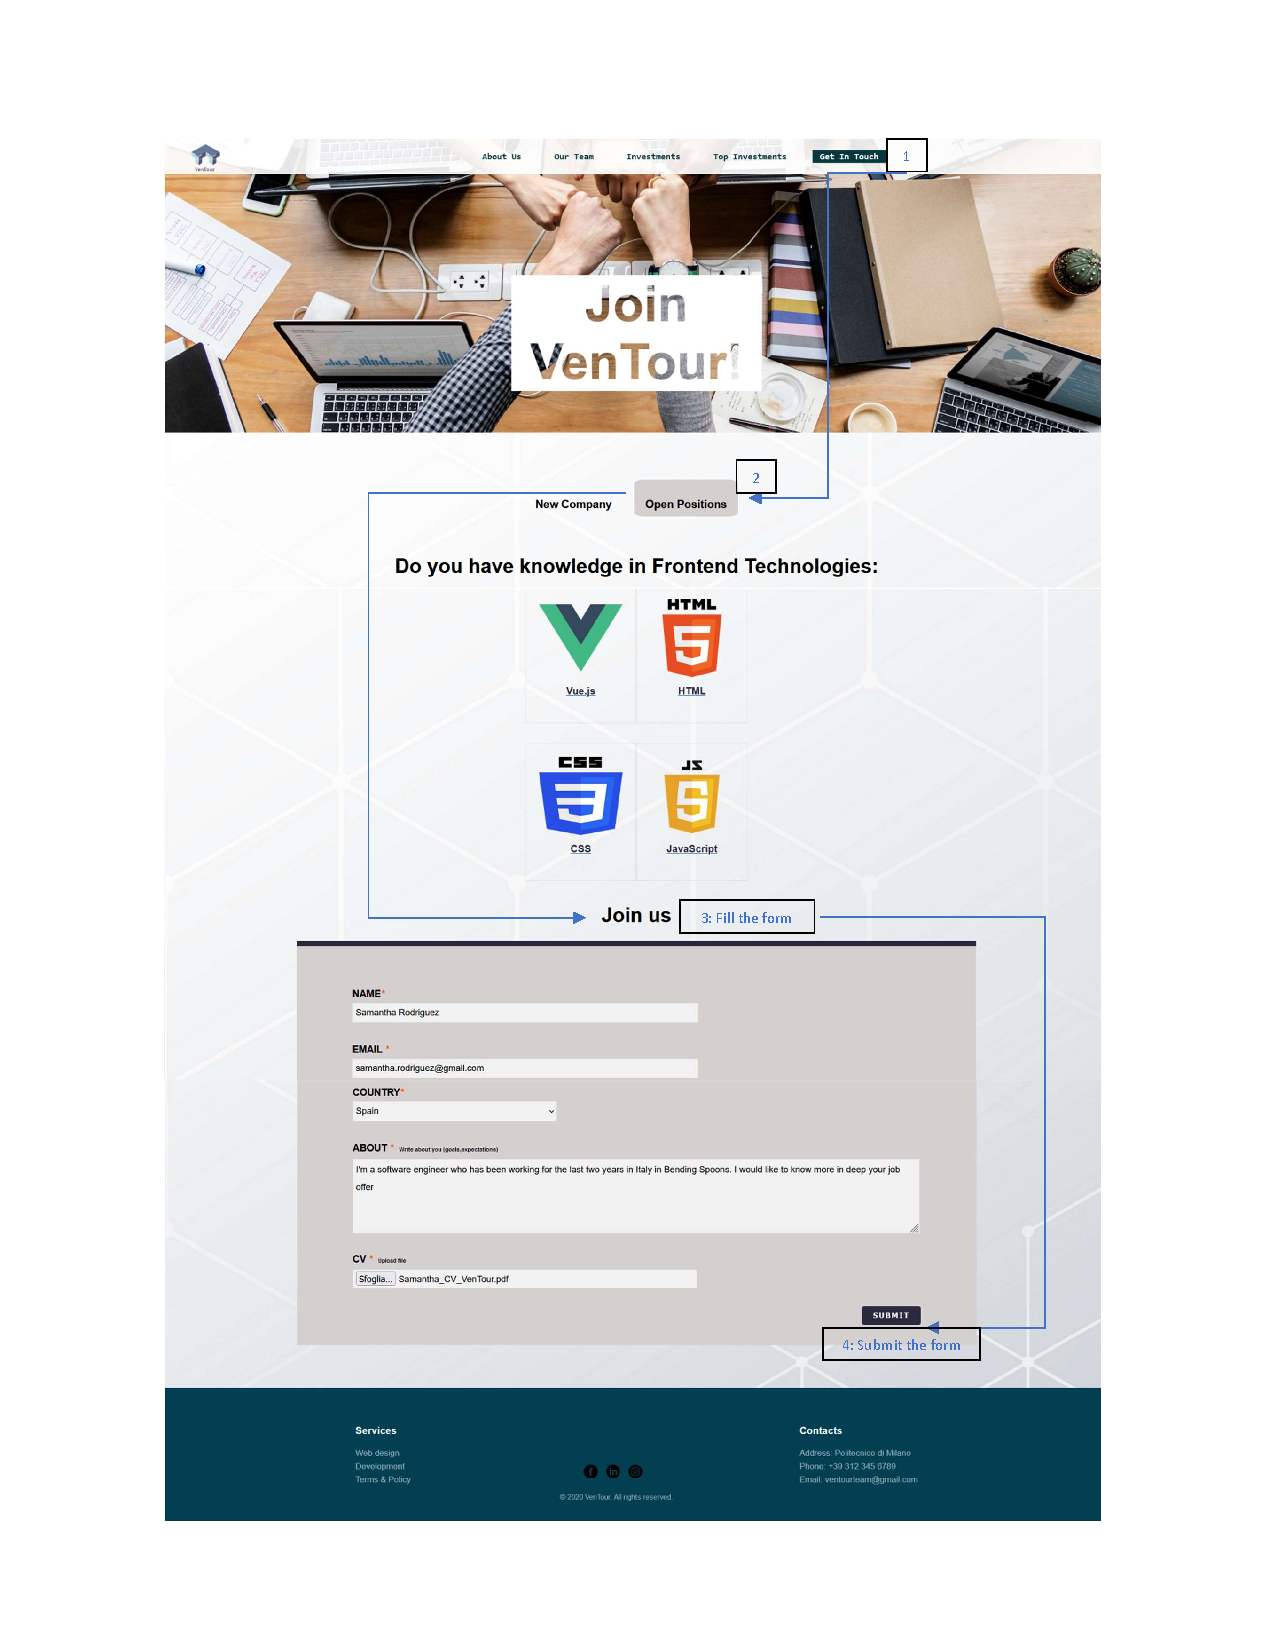
\includegraphics[width=\textwidth]{Images/scenarios/UseCase 2.pdf}
            \caption{Following, Samantha goes in the "Get in touch" page and see what are the open position and applies for one of them}
            \label{fig: UC02}
        \end{figure}

\clearpage
		\subsection{Use case 2}
			Lily is a seasoned entrepreneur who has built and sold successful technology startups in the past 10 years. She is now interested in exploring some other possible investment opportunities in the area of artificial intelligence.\\ Lily found our company from the rankings of "Best Venture Capital Companies of the year" and now wants to explore the companies in which we have invested in, specifically within the area of technology.\\
			She opens the website and looks at the navigation bar, where she finds the tab \textit{Investments}. She clicks on it and starts exploring the page, by first reading the short overview under the title and the instruction marked with \textit{*}. She understands that here she can find the investments she was looking for by using the filter provided. She starts reading the investment areas and finds the \textit{Technology Investments} listed as first area.\\Then she clicks on the filter next to the instruction \textit{"Select \& Check Companies"} and finalizes the filtering by clicking on \textit{Show all} button. (see \ref{fig:scen1-1}) \\ This last button will scroll the page to \textit{Portfolio Snapshot}, showing to Lily all the companies we have invested in the field of Technology.(see \ref{fig:scen1-2})\\ By clicking on each card of the portfolio she explores information about the companies she is interested in. (see \ref{fig:scen1-3})\\ Wanting to make a more informed investment decision she also clicks on \textit{Technology Investments} link and reads general information about our company's  philosophy and commitment in the field of technology (see \ref{fig:scen1-4})
   
   \begin{figure}[!htb]
       \centering
       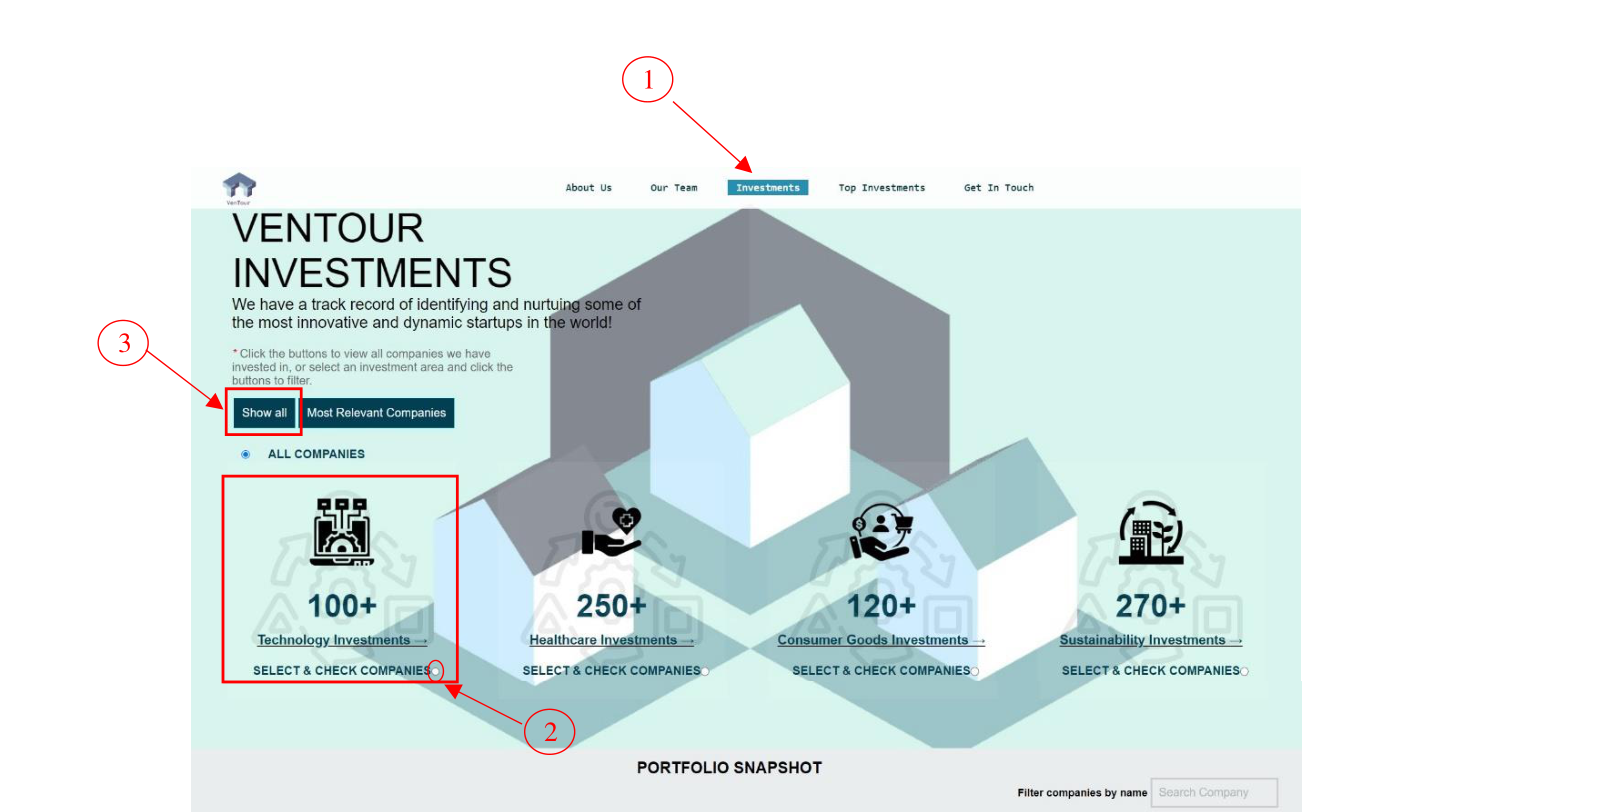
\includegraphics[width=\textwidth]{Images/scenarios/scenario investments1.png}
       \caption{Investments Page first section}
       \label{fig:scen1-1}
   \end{figure}
   
   \begin{figure}[!htb]
       \centering
       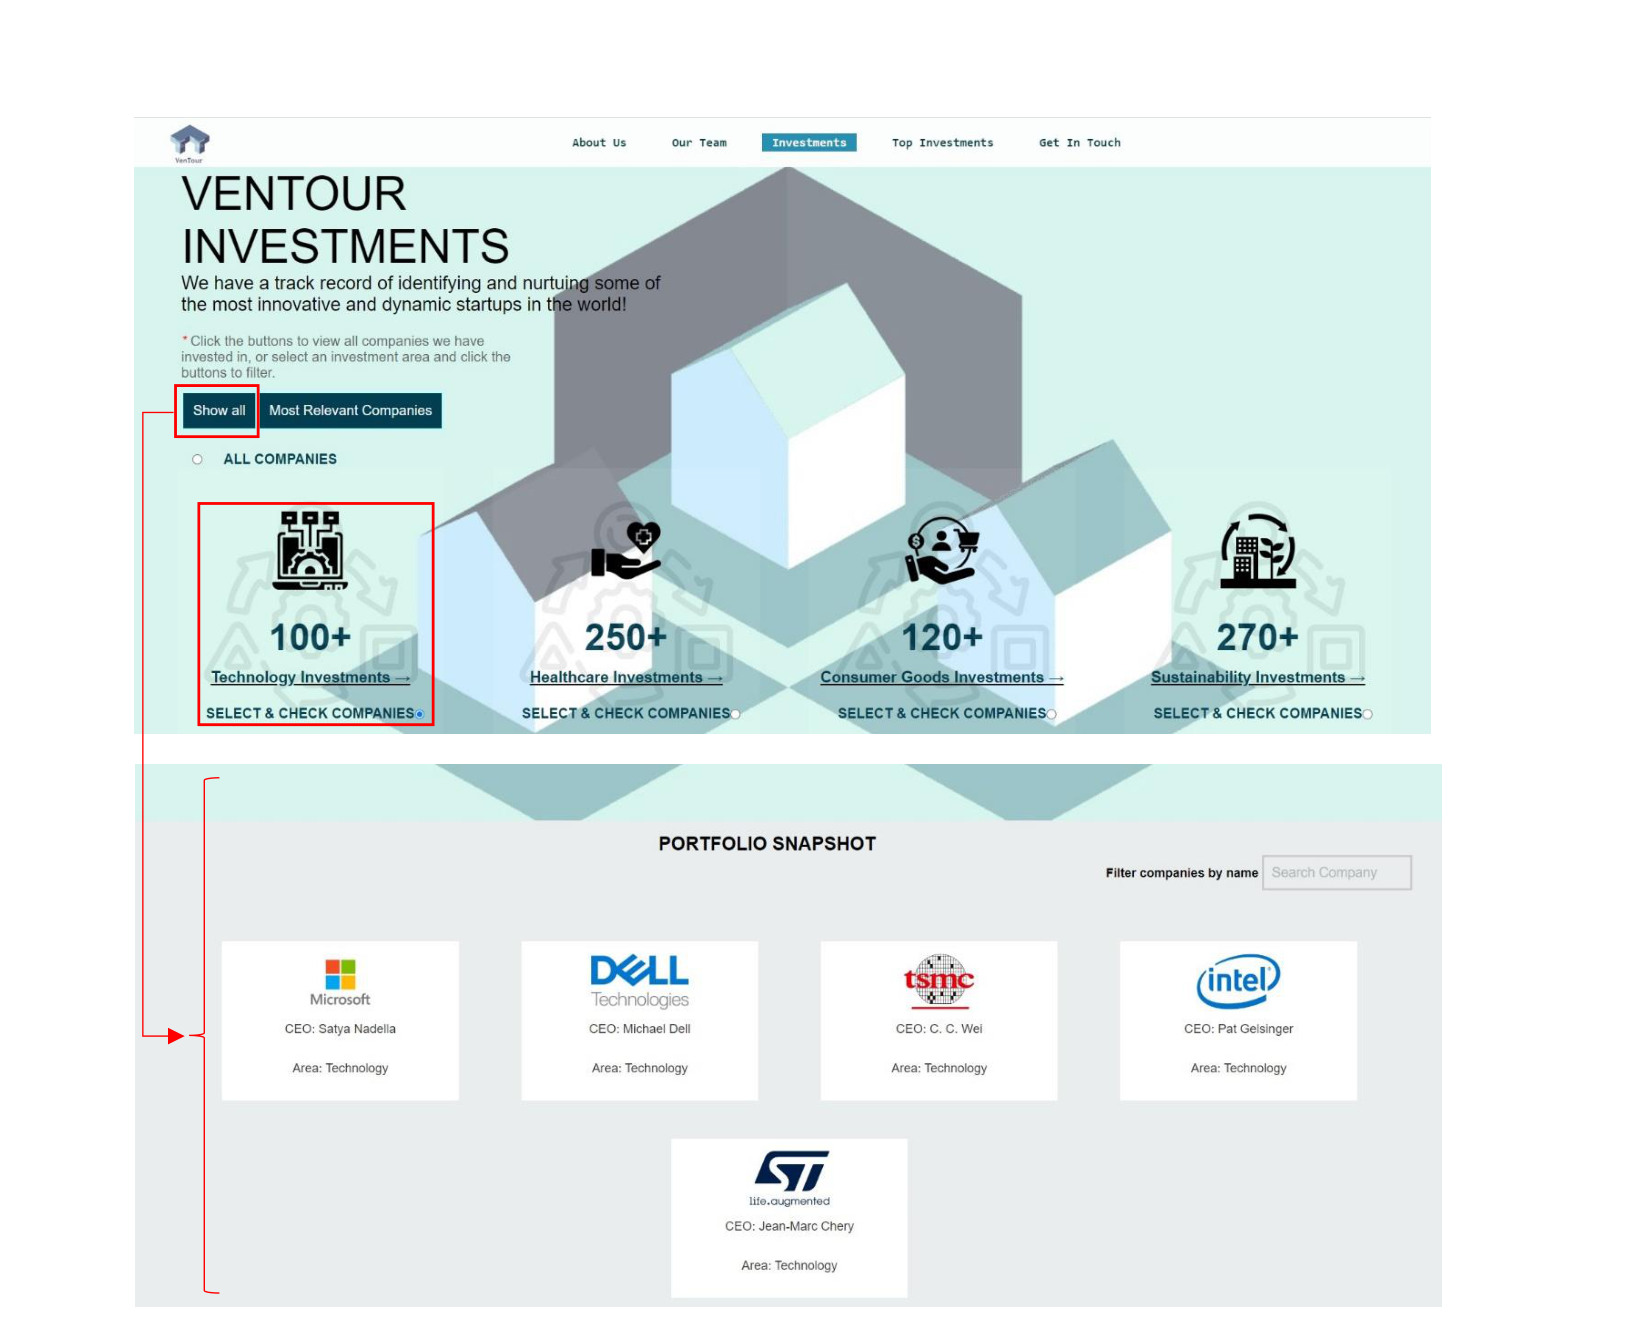
\includegraphics[width=\textwidth]{Images/scenarios/scenario investments2.png}
       \caption{Scrolling to Portfolio Snapshot}
       \label{fig:scen1-2}
   \end{figure}

\begin{figure}[!htb]
       \centering
       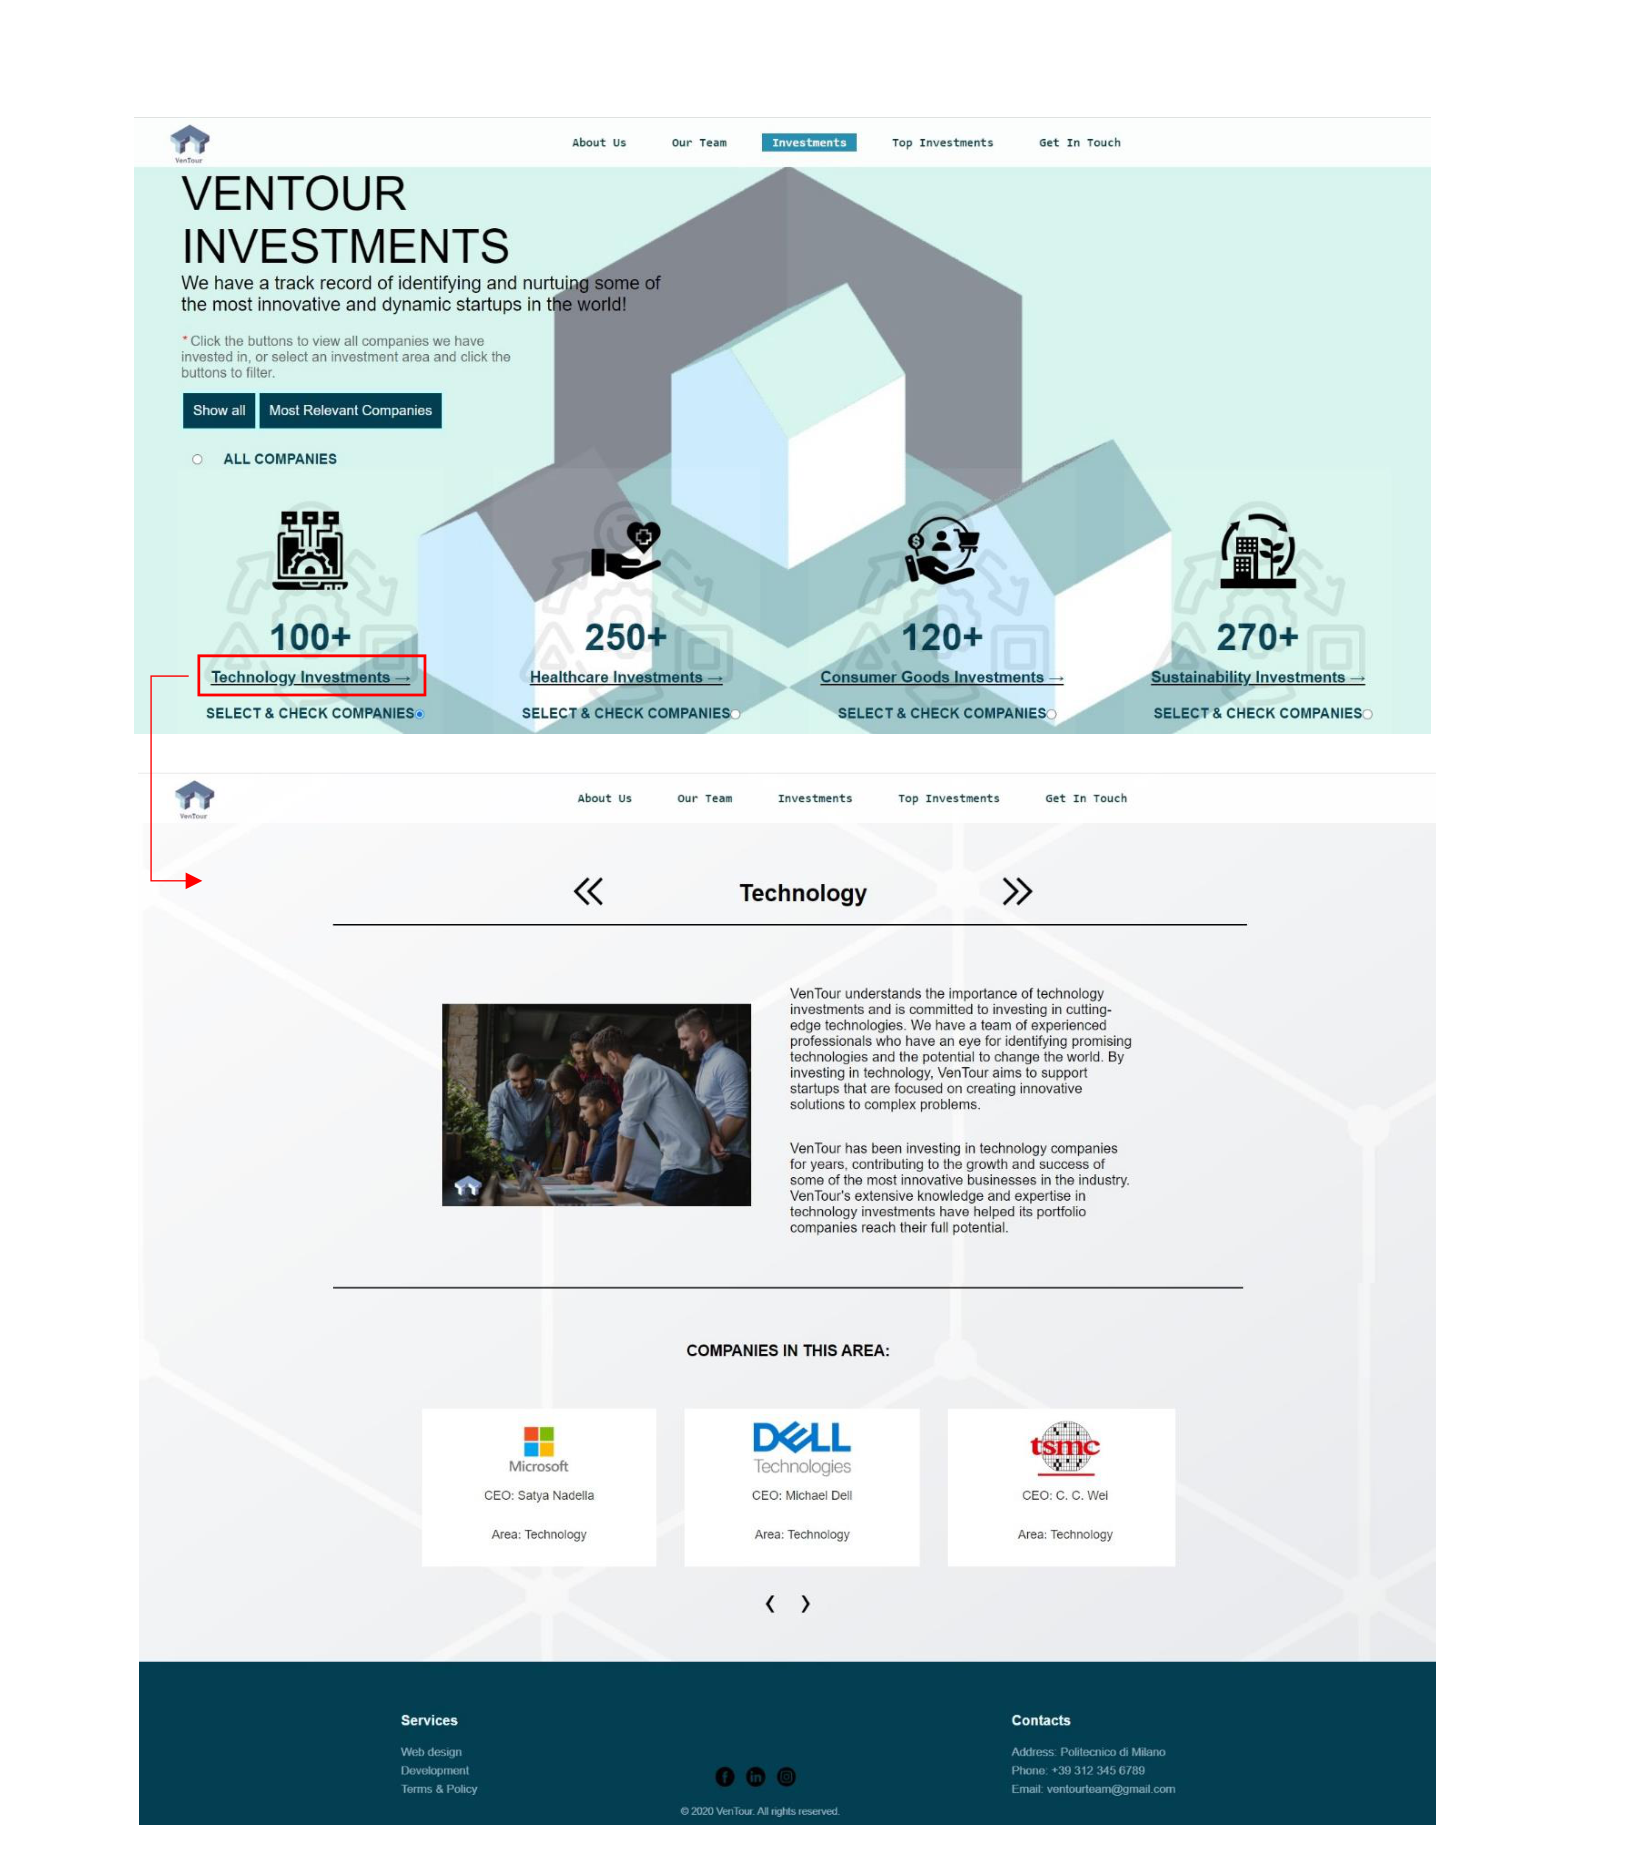
\includegraphics[width=\textwidth]{Images/scenarios/scenario investments3.png}
       \caption{Opening the company page}
       \label{fig:scen1-3}
   \end{figure}

\begin{figure}[!htb]
       \centering
       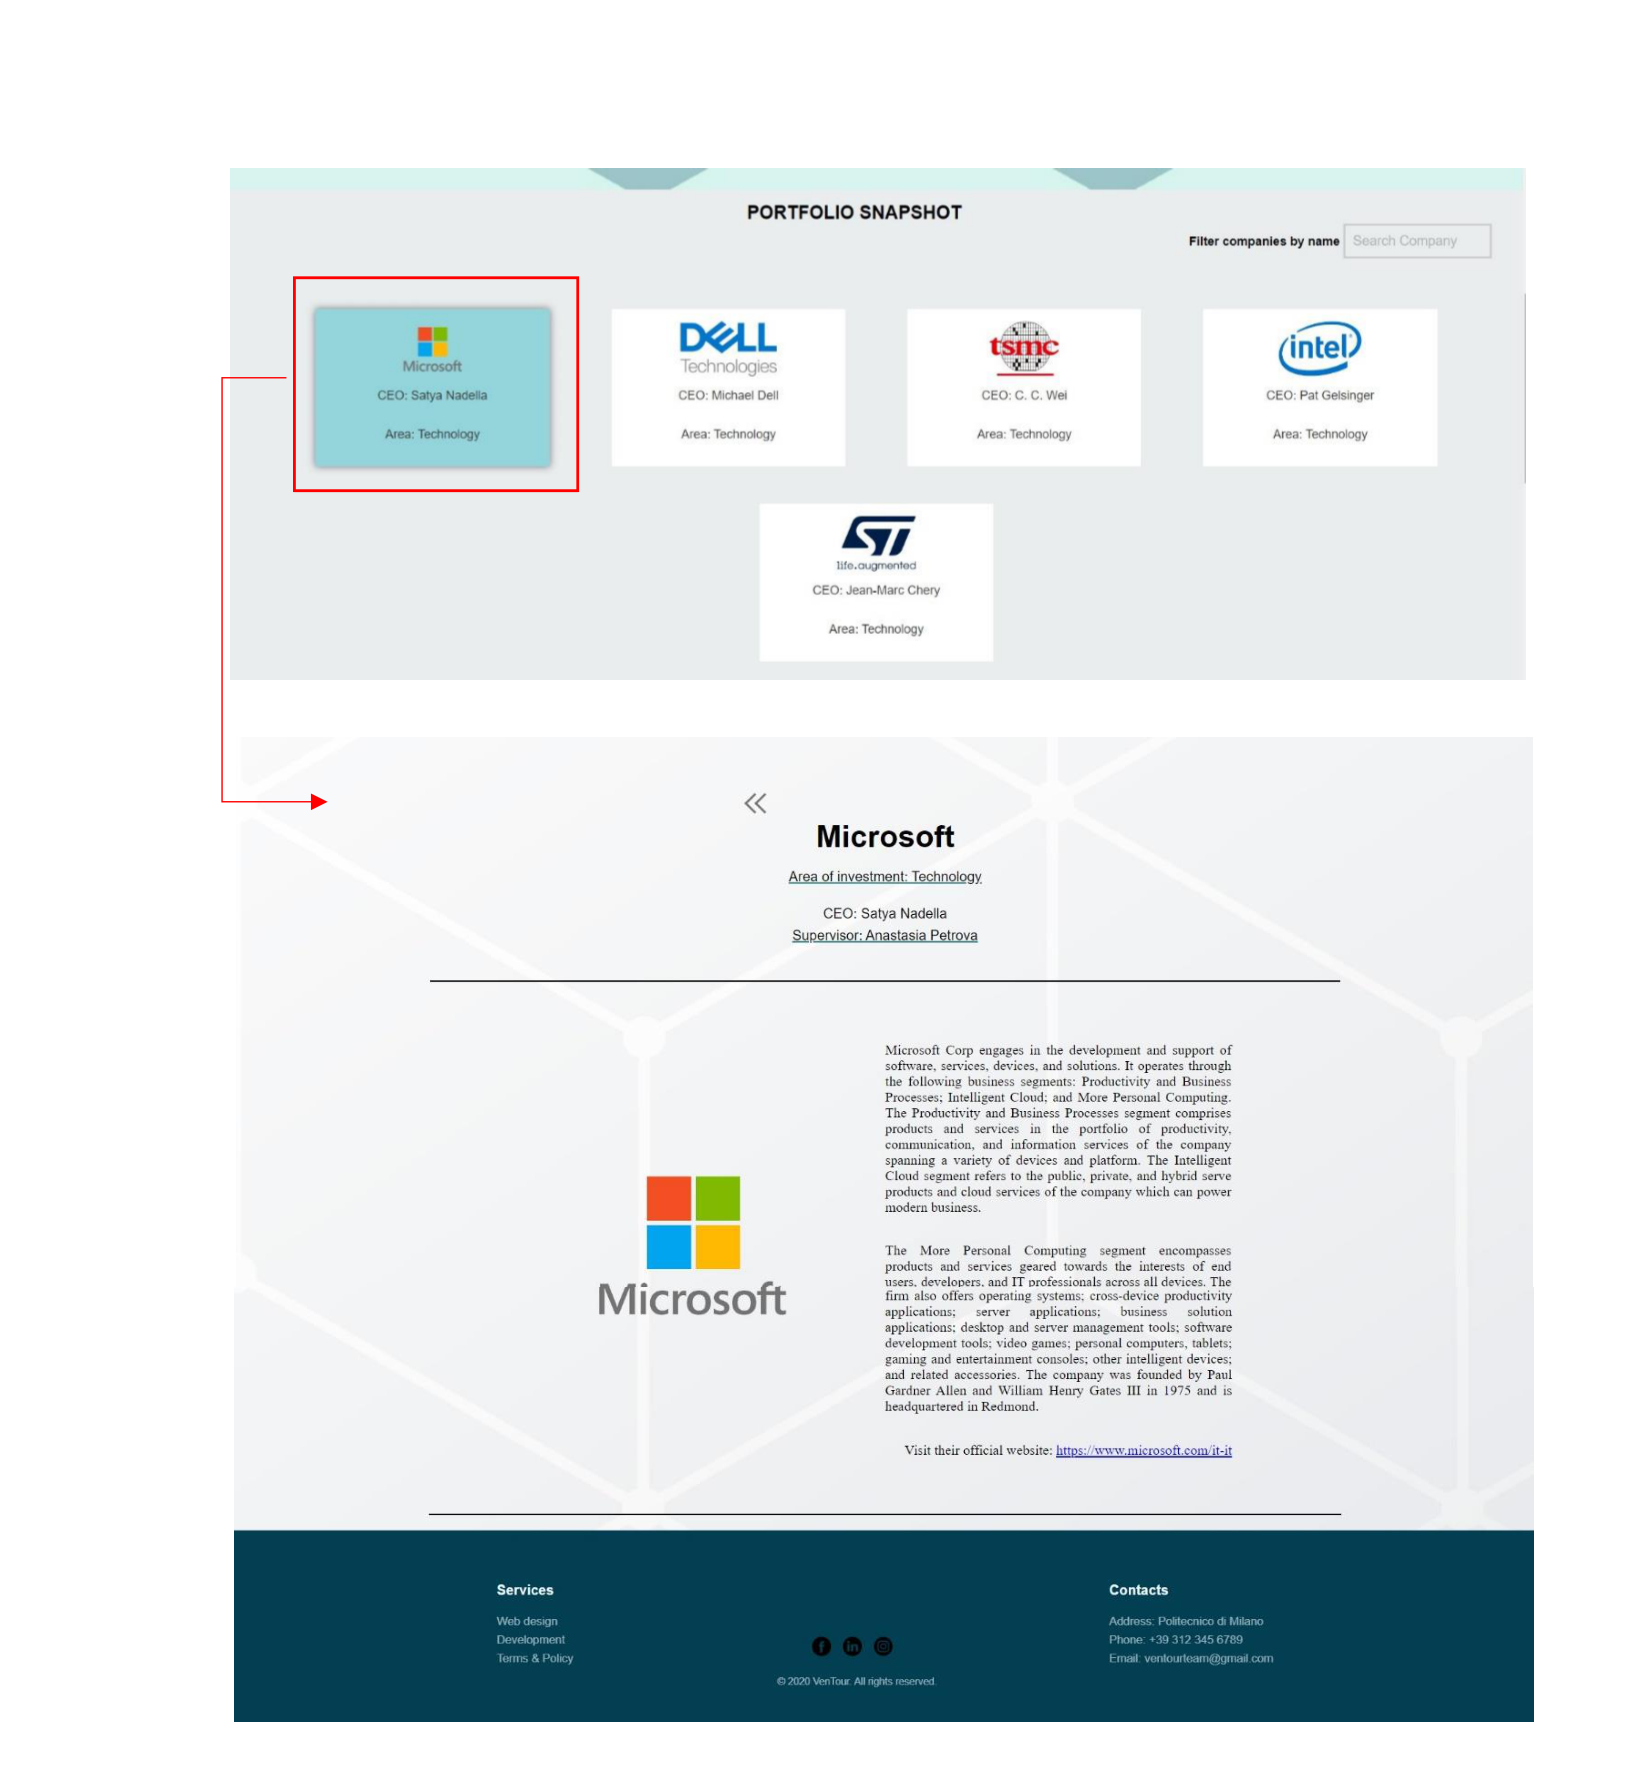
\includegraphics[width=\textwidth]{Images/scenarios/scenario investments4.png}
       \caption{Opening the investment area page}
       \label{fig:scen1-4}
   \end{figure}

  \clearpage

		\newpage
		\subsection{Use case 3}
            Amy is a budding entrepreneur with an innovative idea for a tech startup. She is seeking venture capital funding and is looking for a reliable partner to guide her through the startup journey.\\
            Amy visits \textit{VenTour}'s website to learn more about their expertise, success stories, and the team behind the company. She clicks on "About Us" section to learn about the company history.\\
            Then, convinced by the company's prestigious growth path, she also decided to inquire about the expertise of individual members of the company in the section "Our Team".\\
            After reading the prestigious awards received by the General Manager Anastasia Petrova, Amy gains confidence in \textit{VenTour}'s ability to support her vision and decides to reach out for potential collaboration. To do it, she decides to send an email to the General Manager of VenTour, Anastasia Petrova, by clicking on the dedicated icon.
            
            \begin{figure}[!htb]
                \centering
                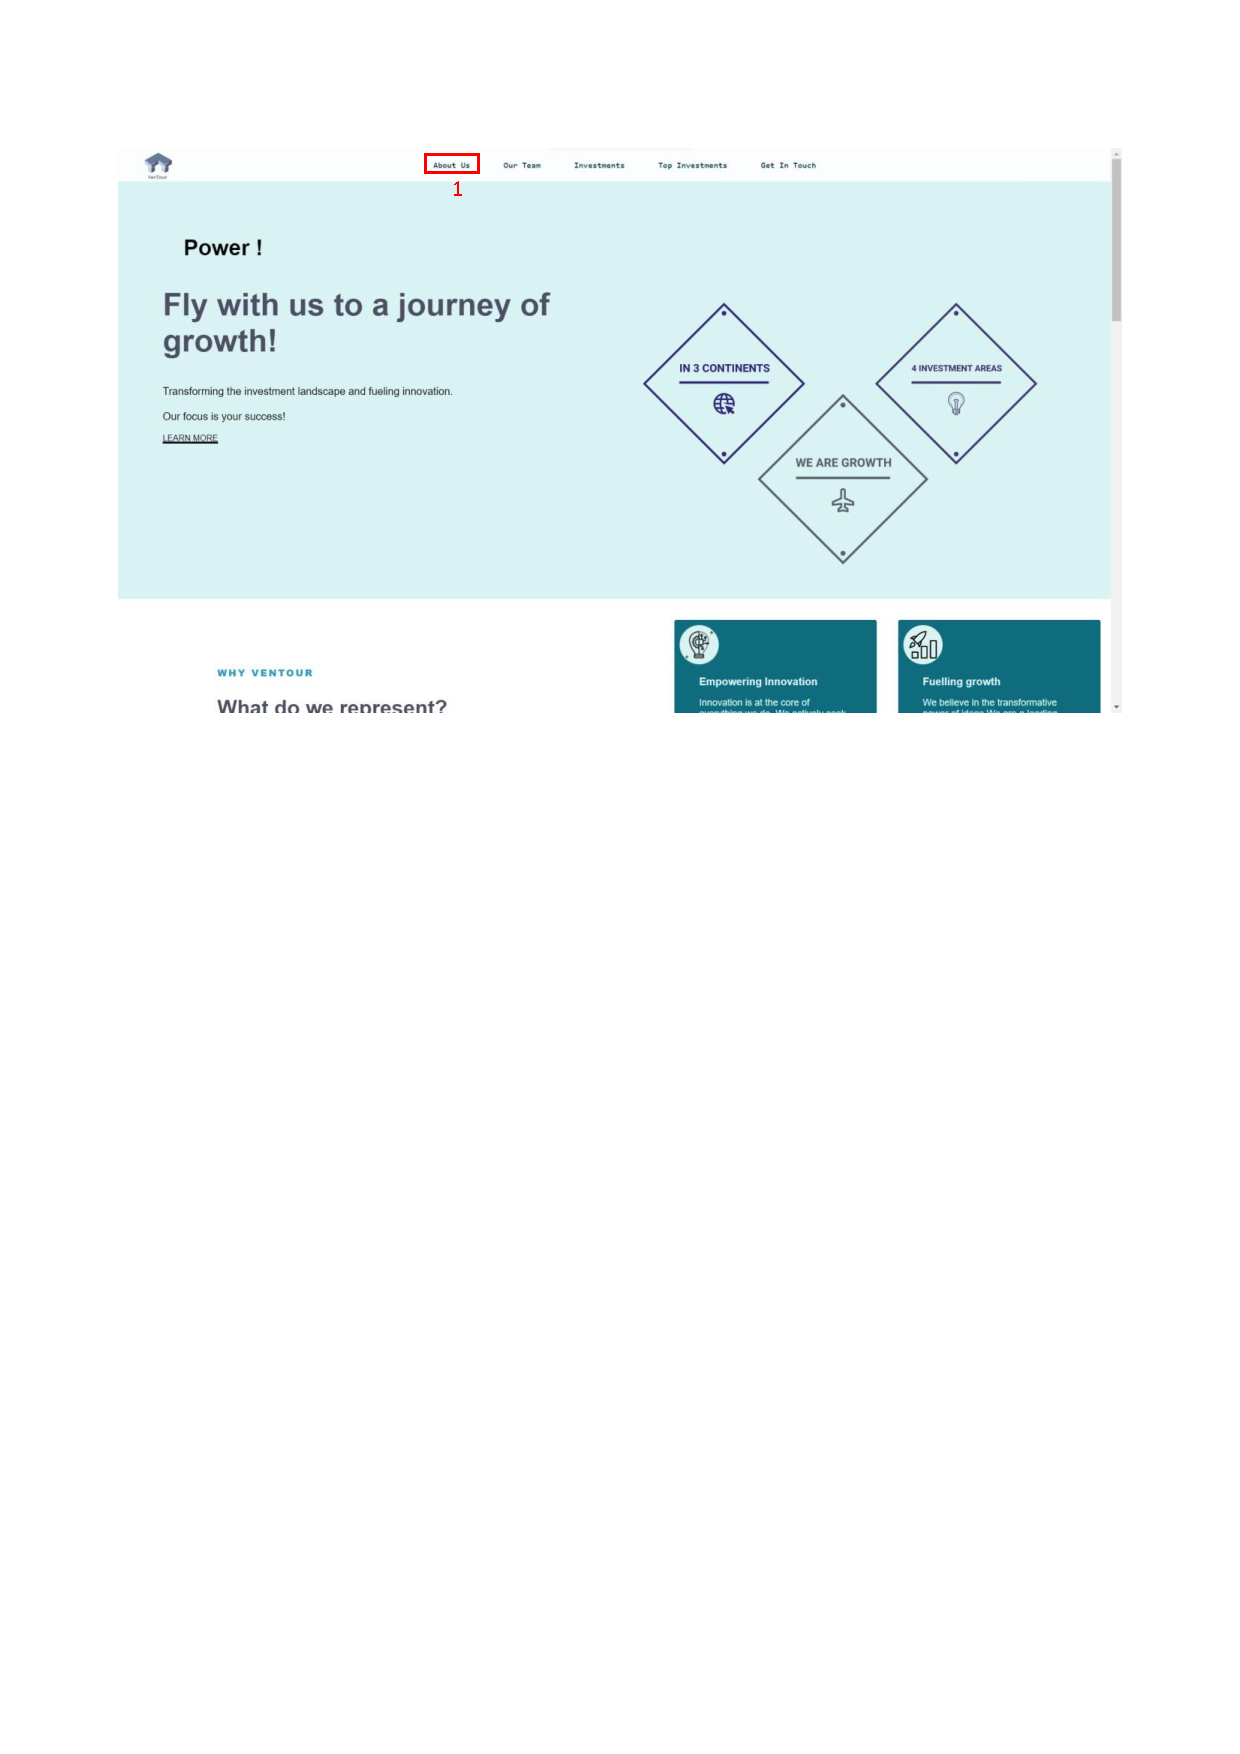
\includegraphics[width=\textwidth, trim=0 450 0 0, clip]{Images/scenarios/use cases 1.pdf}
                \caption{Clicking on "About Us" in Home Page}
                \label{fig:use_cases_3_1}
            \end{figure}

            \begin{figure}[!htb]
                \centering
                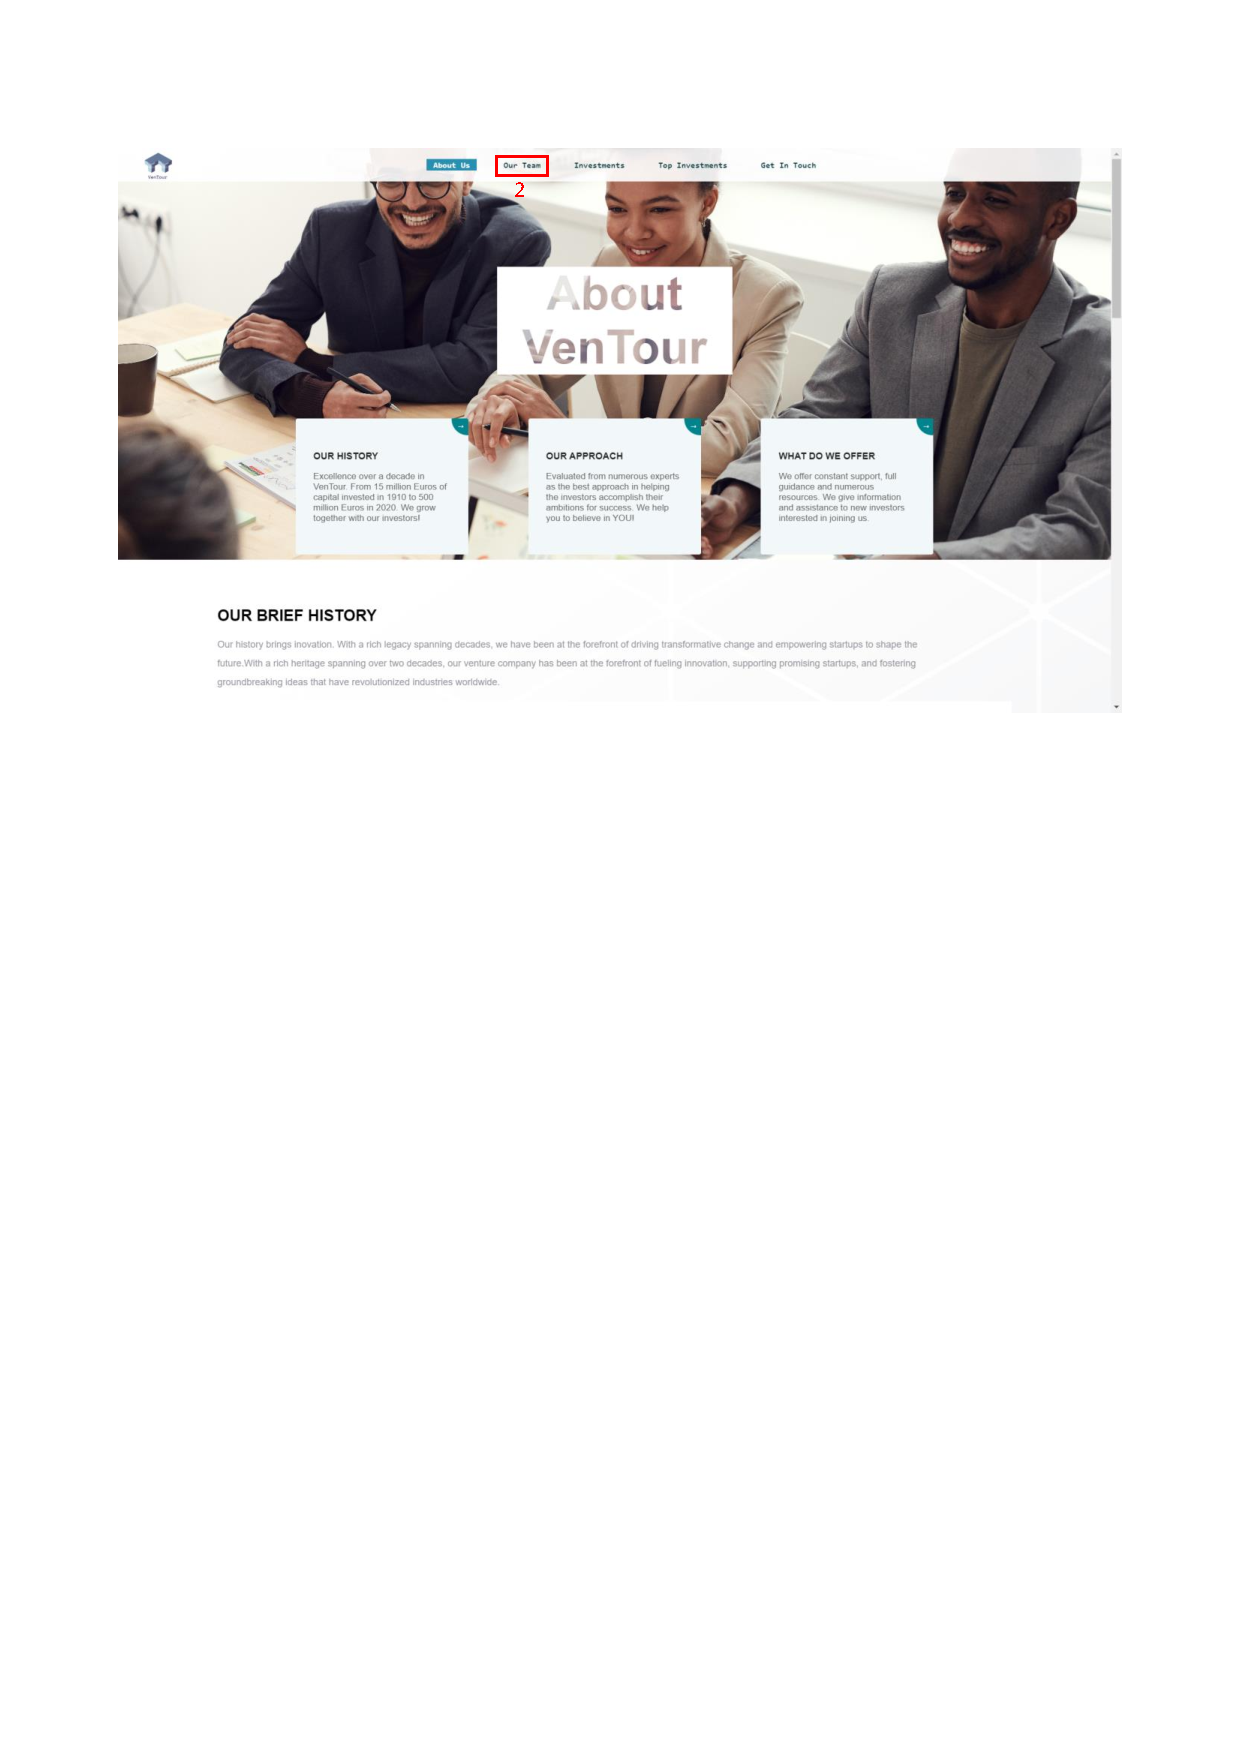
\includegraphics[width=\textwidth, trim=0 450 0 0, clip]{Images/scenarios/use cases 2.pdf}
                \caption{Clicking on "Our Team" in "About Us" page}
                \label{fig:use_cases_3_2}
            \end{figure}

            \begin{figure}[!htb]
                \centering
                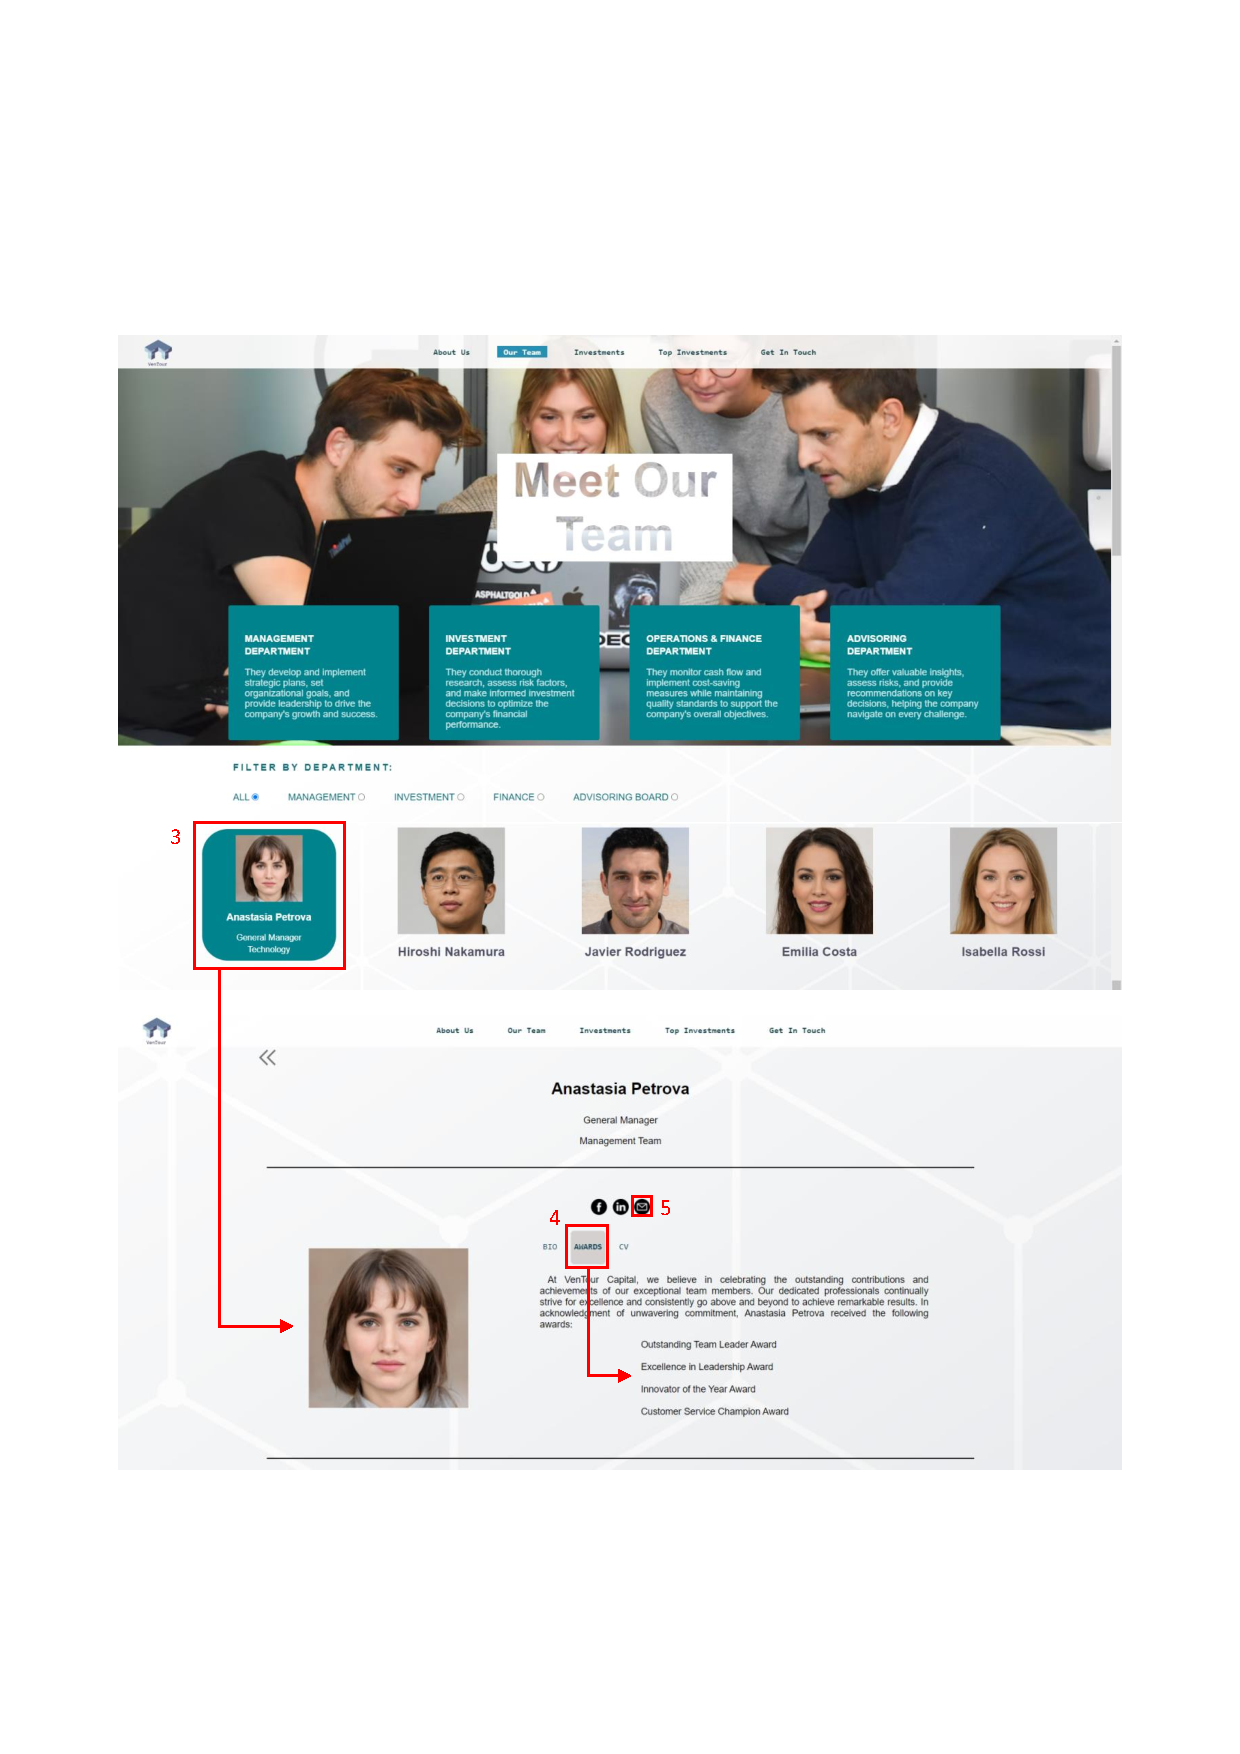
\includegraphics[width=\textwidth]{Images/scenarios/use cases 3.pdf}
                \caption{Exploring General Manager's Award in dedicated page. Contacting Anastasia Petrova by email.}
                \label{fig:use_cases_3_3}
            \end{figure}

\end{document}